\section{Interface}
\vspace{1cm}


Le dernier axe important de la transition numérique qui m’a été confiée, a été la refonte de l’interface de gestion des arbitres et y intégrant les nouveaux outils créés. Il m’a fallu moderniser cette interface en gardant la nouvelle identité du site mise en place par mon tuteur.

Au total, l’interface devait posséder trois pages distinctes pour chacune des fonctionnalités principales de cette partie du site. Celles-ci sont :

\begin{itemize}
    \item L’interface principale pour les désignations des arbitres
    \item Une interface secondaire pour la gestion des habilitations.
    \item Une dernière interface pour la gestion des poules à afficher ou non
\end{itemize}

\vspace{1cm}

\begin{figure}[!h]
    \centering
    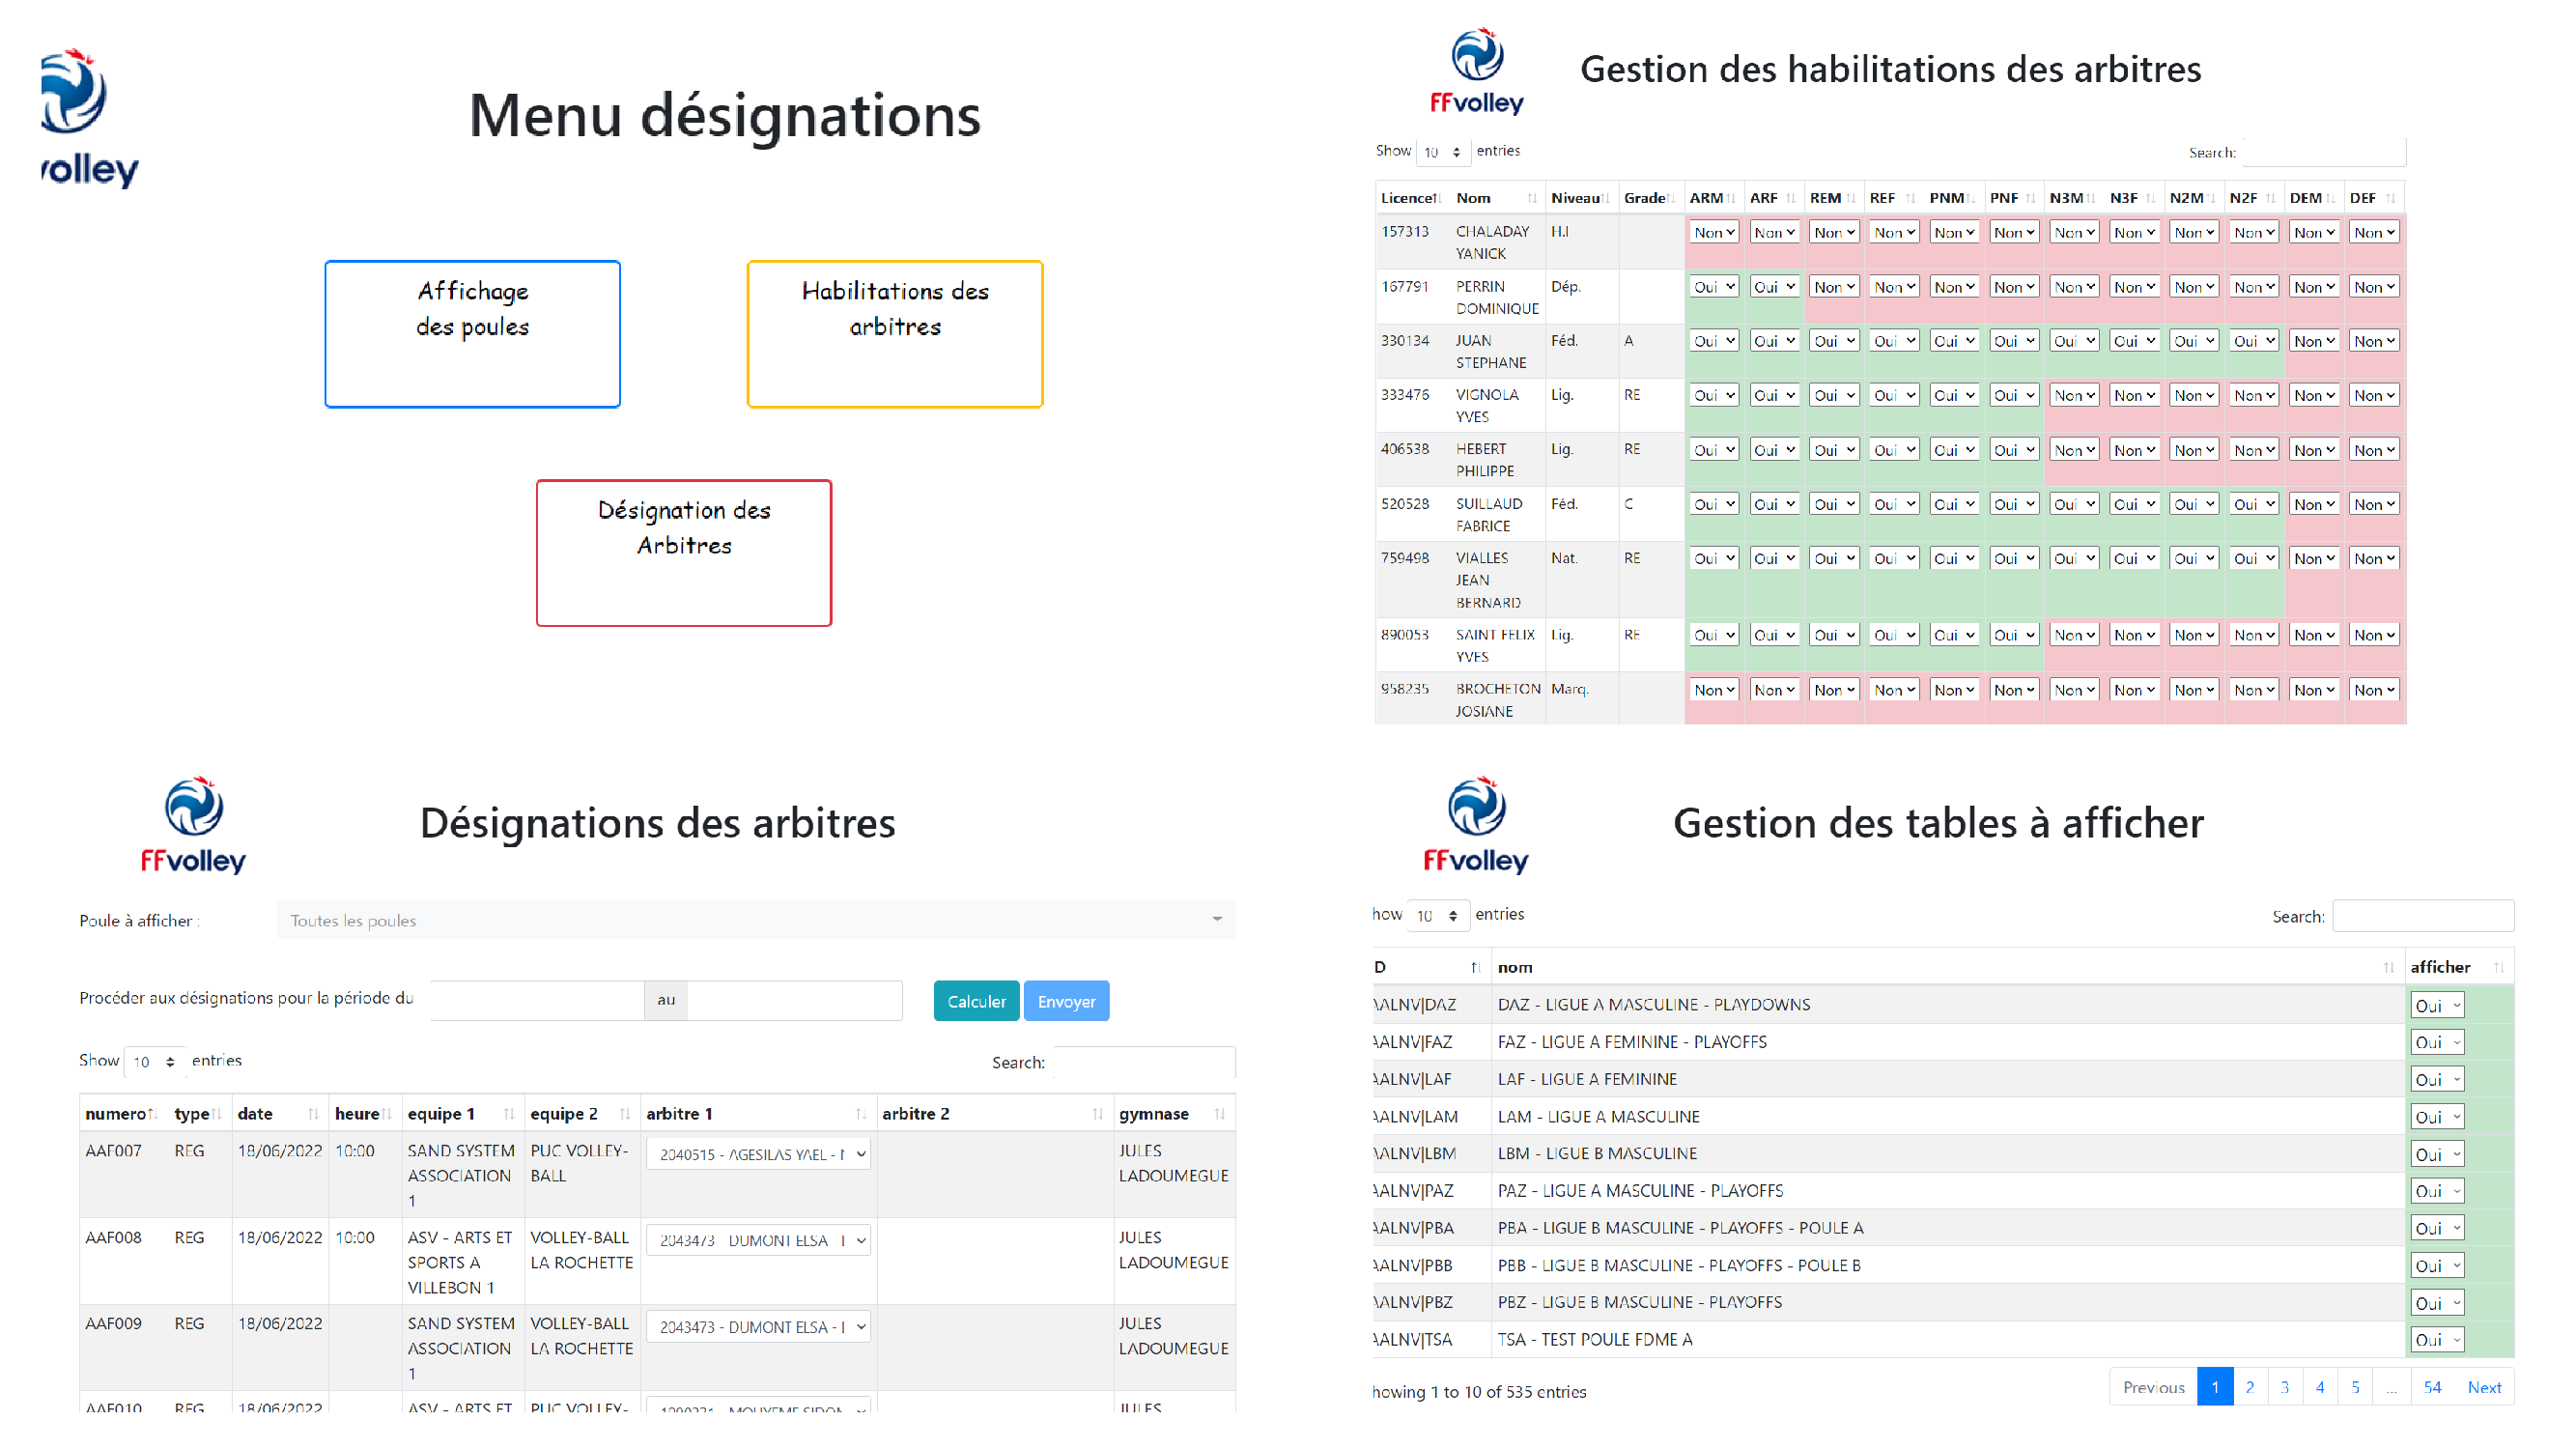
\includegraphics[width=\linewidth]{pages}
    \caption{Les différentes pages de l'interface}
\end{figure}

\vspace{1cm}

Ces interfaces exclusivement composées de tableaux. Ceux-ci devaient faciliter l’expérience utilisateur en intégrant une pagination, un tri par colonne et une barre de recherche.

Heureusement, l’outil \colored{Datatables}  permettait de répondre à l’ensemble de ces contraintes. 
Cet outil basé sur JQuery permet d’intégrer plusieurs fonctionnalités à un tableau html dont la pagination, la barre de recherche et le tri en fonction des colonnes.\\ \\

Pour la réalisation de ces pages, j’ai d’abord procédé au maquettage de l’application avec le logiciel dédié Adobe XD. Le but était de mettre en place un schéma visuel à suivre qui me permettrait de me concentrer uniquement sur l’implémentation du côté technique.

Une fois cette maquette réalisée et validée par mon tuteur, je me suis donc basé sur cette celle-ci pour réaliser mes pages.\\

Pour faciliter le côté responsive, et pour être en accord avec les outils déjà utilisés pour ce projet, j’ai utilisé la librairie Bootstrap pour le côté statique et JQuery pour le côté dynamique. \\

Faisant partie d’un intranet fermé au public, le référencement de ces pages n’était pas une priorité. J’ai cependant tout de même structuré ces pages en exploitant au mieux les balises html de chaque élément composant celles-ci, afin d'exploiter au moins le référencement naturel.